% Created 2020-05-06 mié 13:54
% Intended LaTeX compiler: pdflatex
\documentclass[a4paper, 12pt]{article}
\usepackage[utf8]{inputenc}
\usepackage[T1]{fontenc}
\usepackage{graphicx}
\usepackage{grffile}
\usepackage{longtable}
\usepackage{wrapfig}
\usepackage{rotating}
\usepackage[normalem]{ulem}
\usepackage{amsmath}
\usepackage{textcomp}
\usepackage{amssymb}
\usepackage{capt-of}
\usepackage{hyperref}
\usepackage{float, amsfonts, commath, mathtools}
\author{Tabaré Pérez}
\date{\today}
\title{Lecture 14 - 3: Introduction to the K-Medoids Algorithm}
\hypersetup{
 pdfauthor={Tabaré Pérez},
 pdftitle={Lecture 14 - 3: Introduction to the K-Medoids Algorithm},
 pdfkeywords={},
 pdfsubject={},
 pdfcreator={Emacs 26.3 (Org mode 9.3.6)}, 
 pdflang={English}}
\begin{document}

\maketitle
\textbf{K-MEANS ALGORITHM}

\begin{enumerate}
\item Ramdomly initialize \(z^{(1)} \ldots z^{(K)}\)
\item Iterate unitl no change in cost:
\begin{itemize}
\item 2a. for \(i=1 \ldots n\):

\(C_j = \{i|\) s.t. \(z^{(j)}\) is closest to \(x^{(i)}\}\)

\item 2b. for \(j=1 \ldots K\):

\(z^{(j)} = \frac{\sum_{i \in C_j} x^{(i)}}{\abs{C_j}}\)
\end{itemize}
\end{enumerate}

As I said earlier, K-medoids will be derived almost directly from the K-means
algorithm. Which parts of the algorithm are affected by the fact that our
points, that our representatives are not part of the original points?

So clearly when we are looking at step one, in K-means, whenever we selected
points, we can select any points on the plane.

In this case, because we want our points to be part of the original set, we can
explicitly constrain the first step and say, you still have a freedom to
randomly select whoever you want to be this representative.

But, do select it from the original set of points. This will be the first step
that we may want to change. So let's write it down:

\begin{enumerate}
\item Ramdomly initialize \(\{z^{(1)} \ldots z^{(K)}\} \subseteq \{x^{(1)} \ldots x^{(n)}\}\)
\end{enumerate}

We will say randomly initialize. And we would, again, select this \(z^{(1)} \ldots
z^{(K)}\) in a way that they are part to our set \(x^{(1)} \ldots x^{(n)}\).

So what we wrote down that they have to be some subset of their original points.
So now we selected our representatives to be part of the original cohort.

And we can continue our iterated procedure:
\begin{itemize}
\item 2) Iterate until there is no change in cost:
\end{itemize}

And let's look at step \textbf{2a}. So in step \textbf{2a}, every point had to go and find
itself the closest representative. In this case, this particular step, first of
all, doesn't limit us as to what the representative could be, because we already
selected them. And also, it can work with any distance function, because as far
as you can compute the distance between the representative and a point, it will
work. So we can just directly copy the step \textbf{2a}, which is building the
partitions, given particular representative, directly from what we had before:

\begin{itemize}
\item 2a. for \(i=1 \ldots n\):

\(C_j = \{i|\) s.t. \(z^{(j)}\) is closest to \(x^{(i)}\}\)
\end{itemize}


So our step \textbf{2a} will be for \(i\) from \(1\) to \(n\) and \(C_j\) collects all
of the \(i\)'s such that \(C_j\) is closest to \(x^{(i)}\).

So now the next step for us is actually go and select the new representative.
And what we know, this is the place where all the action will happen, because in
K-means in this step, we were violating both assumptions. First of all, we were
selecting the point which may not necessarily be the member of the original set.
And the second point is the reason our representative looks like a centroid was
because we did this derivation and we directly built on the assumption that our
distance metric happened to be square Euclidean distance.

So here we would expect that the change will happen. And let's just intuitively
see what we would like to get in this step \textbf{2b}. Let's say your cluster looks
like something like this.

\begin{figure}[H]
\centering
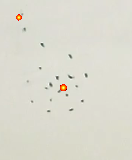
\includegraphics[width=0.25\textwidth]{./pic/u04-l14-03-fig-01.png}
\caption{\label{fig:orgc2cc50d}Intuition}
\end{figure}

In this instance, like, the worst choice that you can make is to select this guy
to be the representative of this partition, because the distance from these guys
to all other points will be very, very high. So ideally, you would select
somebody from here, which is kind of in the middle and close to all the points.

So what we will do now is exactly write in the form of what I just said in
words:

\begin{itemize}
\item 2b. for \(j=1 \ldots K\):

\(z^{(j)} \in \{x^{(1)} \ldots x^{(n)}\} | \sum_{i \in C_j} \text{distance}(x^{(i)}, z^{(j)})\) is minimal.
\end{itemize}

We will go from the cluster \(1\) to cluster \(K\), then we would say, I want to
select point \(z^{(j)}\), and this particular point is going to come from my
original set, from my original points \(x^{(1)}\) to \(x^{(n)}\).

And what would I request from this point?

I am going to select this point that if we are looking at the distance between
this point and all the other members of the group \(i \in C_j\), we would want
this distance to be minimal.

So we will select one of the points from our original cohort such that the sum
of distances from this point to all the members of this cluster is minimal.

So this way, it will work with any distant function you may want to use. And
also, we don't make any assumption about this form because we explicitly are
going to compute the distances between these points and the rest.

\begin{enumerate}
\item Ramdomly initialize \(\{z^{(1)} \ldots z^{(K)}\} \subseteq \{x^{(1)} \ldots x^{(n)}\}\)
\item Iterate until there is no change in cost:
\begin{itemize}
\item 2a. for \(i=1 \ldots n\):

\(C_j = \{i|\) s.t. \(z^{(j)}\) is closest to \(x^{(i)}\}\)

\item 2b. for \(j=1 \ldots K\):

\(z^{(j)} \in \{x^{(1)} \ldots x^{(n)}\} | \sum_{i \in C_j} \text{distance}(x^{(i)}, z^{(j)})\) is minimal.
\end{itemize}
\end{enumerate}

So doing this algorithm, we for sure can solve the two problems which were
limiting for us in the case of K-means:

\begin{itemize}
\item We can work with any distance function.
\item We also are guaranteed to get points from our original set.
\end{itemize}
\end{document}